% !TEX root = ../SCXMLREF.tex

\subsection{iUML-B State-machines}
\label{sec:iumlb}

\iUMLB provides a diagrammatic modelling notation for \EventB in the form of state-machines and class diagrams. The diagrammatic models are contained within an \EventB machine and generate or contribute to parts of it. For example a state-machine will automatically generate the \EventB data elements (sets, constants, axioms, variables, and invariants) to implement the states while \EventB events are expected to already exist to represent the transitions. Transitions contribute further guards and actions representing their state change, to the events that they elaborate. A choice of two alternative translation encodings are supported by the iUML-B tools.  State-machines are typically refined by adding nested state-machines to states.

Figure~\ref{fig:iumlb-sm} shows an example of a state-machine, named |SM|.
\begin{figure}[!htbp]
	\centering
	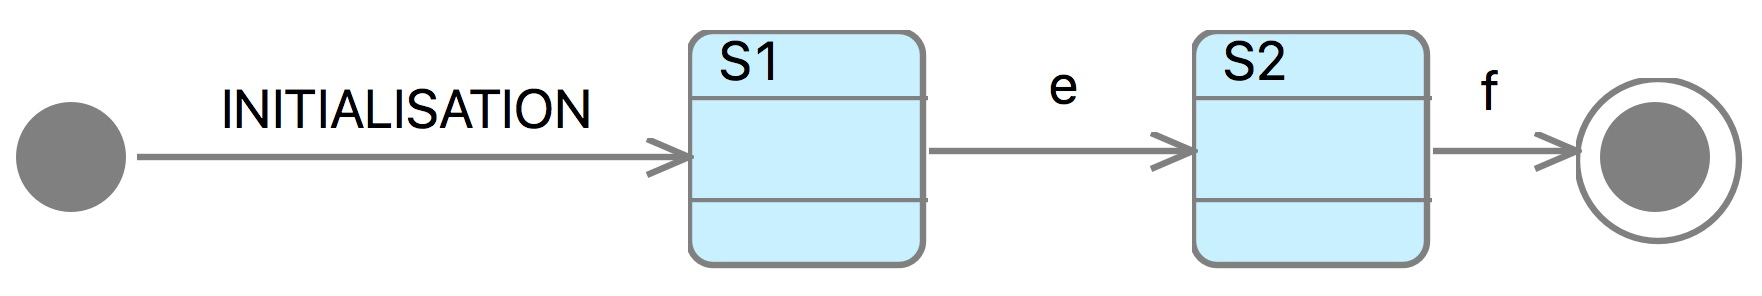
\includegraphics[width=0.8\textwidth]{figures/iumlb-SM}
	\caption{An example \iUMLB state-machine \texttt{SM}}
	\label{fig:iumlb-sm}
\end{figure}
Here we show a translation of state-machine |SM| using the \emph{enumeration} encoding, where each state is encoded as a constant from an enumerated set |SM_STATES|.  Variable |SM|, which represents the current state of the state-machine, is initialised to |S1|. Events |e| and |f| change the value of |SM| according to the transitions in the state-machine.  The \EventB translation can be seen below.
\begin{EventBcode}
sets SM_STATES
constants SM_NULL S1 S2
axioms
    partition(SM_STATES, {SM_NULL}, {S1}, {S2})
variables SM
invariants SM !: SM_STATES
events
    @INITIALISATION: begin SM := S1 end
    @e: when SM = S1 then SM := S2 end
    @f: when SM = S2 then SM := SM_NULL end
end
\end{EventBcode}
	% $\carriersets{\BSMSTATES}$ \Bhspace $\constants{\BSMNULL, \BSI, \BSII}$ \Bvspace
	% $\axioms{\partition(\BSMSTATES, \BSMNULL, \BSI, \BSII)}$ \Bvspace
	% $\variables{\BSM}$ \Bhspace $\invariants{\BSM \in \BSMSTATES}$ \Bvspace
	% $\event{INITIALISATION}{}{}{}{}{\BSM \bcmeq \BSI}$ \Bhspace
	% $\event{\Be}{}{}{\BSM = \BSI}{}{\BSM \bcmeq \BSII}$ \Bhspace
	% $\event{\Bf}{}{}{\BSM = \BSII}{}{\BSM \bcmeq \BSMNULL}$
\KarlaCommented{Colin, the variable encoding description is missing. It should be included for completeness and it is the one we are using at the moment}
%%% Local Variables:
%%% mode: latex
%%% TeX-master: "../SCXMLREF"
%%% End:
